\documentclass[border=4pt]{standalone}
\usepackage{tikz}

\begin{document}
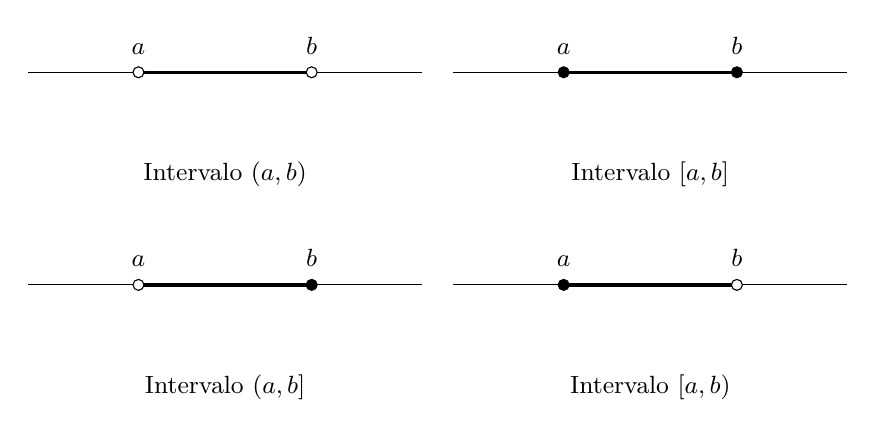
\begin{tikzpicture}[x=1cm, y=1cm, font=\small,
    abierto/.style={circle, draw, fill=white, inner sep=1.4pt},
    cerrado/.style={circle, draw, fill=black, inner sep=1.4pt}]

    % #1 = desplazamiento, #2/#3 = estilo de los extremos, #4 = etiqueta
    \newcommand{\intervalo}[5]{%
        \begin{scope}[shift={#1}]
            \draw (0,0) -- (5,0);
            \draw[very thick] (1.4,0) -- (3.6,0);
            \node[#2] at (1.4,0) {};
            \node[#3] at (3.6,0) {};
            \node[above=3pt] at (1.4,0) {$a$};
            \node[above=3pt] at (3.6,0) {$b$};
            \node at (2.5,-1.3) {Intervalo #4};
        \end{scope}}

    \intervalo{(0,0)}{abierto}{abierto}{$(a,b)$}{}
    \intervalo{(5.4,0)}{cerrado}{cerrado}{$[a,b]$}{}
    \intervalo{(0,-2.7)}{abierto}{cerrado}{$(a,b]$}{}
    \intervalo{(5.4,-2.7)}{cerrado}{abierto}{$[a,b)$}{}

\end{tikzpicture}
\end{document}
